\chapter{Statusseminar}
\section{Baggrund}
Projektets formål er at udvikle en algoritme til kategorisering af lægemiddelskift. På nuværende tidspunkt vurderes kompleksiteten ved lægemiddelskift af ATC-eksperter og er derfor meget personafhængig. En algoritme kan derfor anvendes som et hjælpemiddel til ATC-eksperterne til at vejlede i hvilke tilfælde de skal være særligt opmærksomme på et lægemiddelskift. Med særligt opmærksomme menes der hvilke tiltag eller informationer, som skal videregives til klinikken ved implementeringen af et lægemiddelskift med henblik på at forebygge medicineringsfejl. 

\section{Problemanalyse}
Den stigende andel af ældre, forekomsten og varigheden af kroniske sygdomme samt udviklingen i sundhedsforventninger og teknologier er skyld i stigende sundhedsudgifter i flere europæiske lande~\citep{Ess2003}. Siden år 2007 til 2015 har udgifterne til sygehusmedicin steget 7,8~\% i gennemsnit om året~\citep{Sundhed2016}.

For at begrænse udgifterne har Amgros, Regionernes lægemiddelorganisation, siden år 2007 sendt lægemidler i udbud årligt med henblik på at indkøbe lægemidler af høj kvalitet til bedst mulige pris til de offentlige danske hospitaler~\citep{Sygehusapoteket2017}. Udbud forekommer på lægemidler, hvor der findes mere én leverandør, hvormed lægemidler bringes i konkurrence, hvilket kan give anledning til et kontraktskift~\citep{Amgros2015}. 

Kontraktskift medfører substitution af lægemidler, hvilket betyder udskiftning af et lægemiddel til et andet~\citep{DanskSelskabforPatientsikkerhed2009}. 
Generisk substitution, hvor to lægemidler indeholder samme virksomme stof, er den hyppigste form for substitution. Denne form kræver ikke recept og kan varetages af en sygeplejerske.~\citep{DanskSelskabforPatientsikkerhed2009} 

Der er patientsikkerhedsmæssige konsekvenser forbundet med generisk substitution, herunder fejlmedicinering~\citep{Hakonsen2010}. 
Den hyppigste fejl ved generisk substitution skyldes i 82,1~\% af tilfældene forkert lægemiddel~\citep{Hakonsen2010}. De typiske anledninger til forket lægemiddel er forveksling af emballager eller navne, hvilket i nogle tilfælde har medført forlænget indlæggelse, forværret sygdom og dødsfald~\citep{DanskSelskabforPatientsikkerhed2009}. Lægemidlets implementering ved skift er essentielt i forhold til forebyggelse af medicineringsfejl.  

Informationssystemer har påvist at være anvendeligt i forebyggelsen af medicineringsfejl~\citep{Agrawal2009}. Dette indebærer f.eks. computerbaseret lægeordreindgang, automatisk dispenseringsskabe, bar-kodet medicin administration samt elektronisk afstemning af medicin.~\citep{Agrawal2009} Klinisk beslutningsstøtte, som f.eks. i form af advarsler, har påvist at forbygge forveksling af navn og styrke og ligeledes at reducere antallet af medicineringsfejl~\citep{Campmans2018}.

\section{Data}
Data er indsamlet af Amgros og Sygehusapoteket Region Nordjylland og består af flere excelark, hvor data skal udtrækkes fra og indgå i algoritmen. Forskellige features vægtes alt efter hvor kompleks håndteringen af lægemiddelskiftet er. Denne vægtning er foretaget i samarbejde med en ekspert på området. Følgende features skal anvendes i algoritmen: 
\begin{enumerate}
\item \label{1} \textbf{Navneændring}: Dette kan give anledning til forvekslinger, hvorved den forkerte medicin kan dispenseres.
\begin{enumerate}
\item \textbf{Sound-a-like}: Ved navneændring ønskes der at beregne Levenshtein distancen for at kunne sammenligne om det nye navn er fuldstændig ændret og/eller ligner et allerede eksisterende navn. Et fuldstændig ændret navn kan give anledning til at personalet tager fejl af lægemidlet og derved kommer til at dispensere det forkerte. Et lignende navn skal kombineres med dispenseringsform, så hvis lægemidlet har et lignende navn og samme dispenseringform kan dette give anledning til at det forkerte lægemiddel dispenseres.
\end{enumerate} \vspace{2mm}
\item \textbf{Styrke og  dispenseringsform}: Samme begrundelse som ved punkt \ref{1}. Disse vægtes dog højere end navneændring, da styrke og dispenseringsform kan medføre større komplikationer, hvis der skabes forvirring over disse. \vspace{2mm}
\item \textbf{Analogskift:} Analog substitution er lægemidler med beslægtet kemi og ensartet klinisk virkning. Disse adskiller sig fra generiske som har nøjagtig samme indholdsstof. Der skal være særlig opmærksomhed på disse da det kan være vanskeligt at forudsige individuelle forskelle i virkning og bivirkninger herunder interaktioner mellem lægemidler. \vspace{2mm}
\item \textbf{Risikolægemidler}: Disse lægemidler kan være problematiske, hvis de ender i restordre, altså at lægemidlet ikke kan leveres og det derfor er nødvendigt at finde et erstatningslægemiddel. Disse lægemidler bør være på lager, da det er svært at finde erstatninger for disse samt risikoen for fejl øges ved erstatning.
%Lina: Jeg ved ikke helt om dette skal med, tænker måske det forvirre dem mere, da det omhandler restordre lige pludselig eller kan jeg omformulere mig her? Måske skrive udsolgt/leveringssvigt i stedet for restordre? Hvad tænker du? Er også selv lidt i tvivl hvad begrundelsen for dette er - er det fordi det vil være svært at få et lignende lægemiddel - er det et dyrt område eller hvorfor er disse problematiske?}
\vspace{2mm}
\item \textbf{Komplekse ATC-koder}: Der er nogle ATC-koder som er mere komplekse end andre. Dette er f.eks. på områder som indgår i produktionen på Sygehusapoteket Region Nordjylland og væsker, hvor en ændring i leverandør typisk vil forårsage ændringer af device, hvilket kan skabe problemer i klinikken. 
 \vspace{2mm}
\item \textbf{Medicinråd}: En lille del af lægemidler omhandler medicinrådets behandlingsvejledninger. Disse lægemidler omfatter enkelte hospitalsafdelinger og kræver et tæt samarbejde med disse. Det ønskes ligeledes at lægemidlet implementeres hurtigt, da det er muligt at opnå store besparelser. \vspace{2mm}
\item \textbf{Pris}: Pris er vigtigt i forhold til at opnå besparelser. Det skal ligeledes vægtes om det kan betale sig at skifte et lægemiddel med mindre besparelse, da udskiftningen kan få store betydninger for klinikken i forhold til arbejdsgangen og i værste tilfælde medføre patientsikkerhedsmæssige konsekvenser. \textit{Det er endnu ikke besluttet, hvordan denne faktor skal indgå i algoritmen.}\vspace{2mm}
\end{enumerate}

\section{Algoritme}
Algoritmen vil opbygges på baggrund af et regel-baseret system. %Regel-baseret systemer er nyttige og effektive på områder som kræver symbolsk behandling af viden~\citep{Ligeza2006}.
Udviklingen af regel-baseret system er baseret på fem trin~\citep{Ligeza2006}, som er fremgår af Figur \ref{fig:metode}.  

\begin{figure}[H]\centering	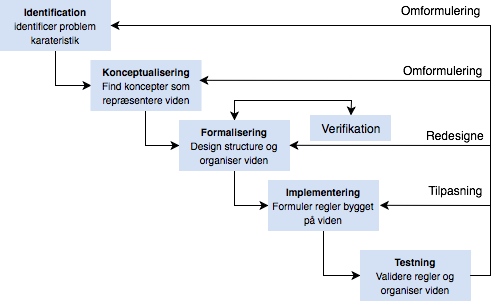
\includegraphics[width=0.7\textwidth]{Statusseminar/metode.png} 
	\caption{De fem trin for udviklingen af regel-baseret system.~\citep{Ligeza2006}}
	\label{fig:metode}  
\end{figure}
\vspace{-0.5cm}
Første trin omhandler identificering af problemer som systemet skal løse, herunder data som systemet skal arbejde på og tilgængelige ressourcer~\citep{Ligeza2006}. Det andet trin er omhandler identificering af nøglekoncepter samt relationer mellem disse som f.eks. typer af data, informationsstrøm og underliggende stukturer. Tredje trin involverer forståelse, beskrivelse og formalisering af problemet og hvordan løsninger findes. Denne proces bør omfatte verificering af systemet. Det fjerde trin har til formål at implementere den formaliseret viden i et program. Det sidste trin omfatter test ved validering af regler og implementeringen.~\citep{Ligeza2006}
 
\section{Samarbejde}
Projektet er et ekstern samarbejde med Sygehusapoteket Region Nordjylland. I projektet samarbejdes med en MedIS-studerende på kandidatuddannelsen Translationel Medicin, som udarbejder spørgeskema og fokusgruppeinterview i forhold til at vurdere, hvornår et lægemiddelskift er kompleks. Disse interview skal danne grundlag for features og vægtning som anvendes i algoritmen. 

Parallelt med dette er et lignede projekt i gang på Sygehusapoteket Region Nordjylland omkring implementeringen af lægemiddelskift, hvor målet er at lave beskrivelser for proceduren for hvordan forskellige typer af lægemiddelskift skal håndteres. Hvormed en algoritme til kategorisering af lægemiddelskift kan være brugbart i denne sammenhæng. 

\section{Projektplan}
På nuværende tidspunkt i projektet arbejdes der på det tredje trin, jævnfør Figur \ref{1} med henblik på snart at indlede fjerde trin. Parallelt med udviklingen af algoritmen arbejdes der på indsamling af viden på forskellige områder i forhold til problemanalysen samt metode.



